\documentclass[11pt]{article}
\usepackage{geometry}                
\geometry{letterpaper}  
                 
\usepackage{graphicx}
\usepackage{amssymb}
\usepackage{epstopdf}
\usepackage{natbib}
\usepackage{amssymb, amsmath}
\usepackage{enumitem}
\setlist[description]{leftmargin=\parindent,labelindent=\parindent}
\DeclareGraphicsRule{.tif}{png}{.png}{`convert #1 `dirname #1`/`basename #1 .tif`.png}

%\title{Circle of Life}
%\author{Patrick Misteli, Ruben K{\"a}lin}
%\date{date} 

\begin{document}



\thispagestyle{empty}

\begin{center}
\includegraphics[width=5cm]{ETHlogo.eps}

\bigskip


\bigskip


\bigskip


\LARGE{ 	Lecture with Computer Exercises:\\ }
\LARGE{ Modelling and Simulating Social Systems with MATLAB\\}

\bigskip

\bigskip

\small{Project Report}\\

\bigskip

\bigskip

\bigskip

\bigskip


\begin{tabular}{|c|}
\hline
\\
\textbf{\LARGE{Circle Of Life}}\\
%\textbf{\LARGE{}}\\
\\
\hline
\end{tabular}
\bigskip
\\
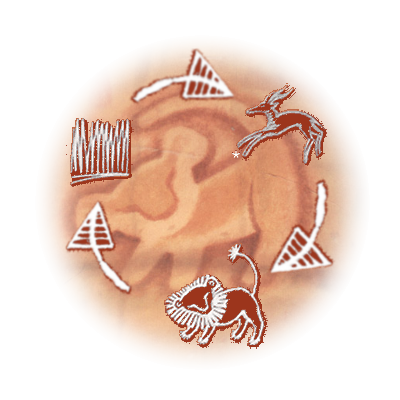
\includegraphics[scale=0.69]{images/circleEdited.png}\\
\bigskip
\LARGE{Patrick Misteli \& Ruben K{\"a}lin}

\bigskip

\bigskip

\bigskip

\bigskip

\bigskip

\bigskip

Zurich\\
May 2014\\

\end{center}



\newpage

%%%%%%%%%%%%%%%%%%%%%%%%%%%%%%%%%%%%%%%%%%%%%%%%%

\newpage
\section*{Agreement for free-download}
\bigskip


\bigskip


\large We hereby agree to make our source code for this project freely available for download from the web pages of the SOMS chair. Furthermore, we assure that all source code is written by ourselves and is not violating any copyright restrictions.

\begin{center}

\bigskip


\bigskip


\begin{tabular}{@{}p{3.3cm}@{}p{6cm}@{}@{}p{6cm}@{}}
\begin{minipage}{3cm}

\end{minipage}
&
\begin{minipage}{6cm}
\vspace{2mm} \large Patrick Misteli

 \vspace{\baselineskip}

\end{minipage}
&
\begin{minipage}{6cm}

\large Ruben K{\"a}lin

\end{minipage}
\end{tabular}


\end{center}
\newpage

%%%%%%%%%%%%%%%%%%%%%%%%%%%%%%%%%%%%%%%



% IMPORTANT
% you MUST include the ETH declaration of originality here; it is available for download on the course website or at http://www.ethz.ch/faculty/exams/plagiarism/index_EN; it can be printed as pdf and should be filled out in handwriting


%%%%%%%%%% Table of content %%%%%%%%%%%%%%%%%

\tableofcontents

\newpage

%%%%%%%%%%%%%%%%%%%%%%%%%%%%%%%%%%%%%%%



\section{Abstract}
In the film "Lion King" from Disney the main character's father explains to his son the concept of what he calls "the circle of life" and how all animals in the food chain hierarchy are needed in order for every species to survive. He abstracts the concept by explaining that lions become grass after they die. This grass is eaten by the antelopes, which are again eaten by the lions to complete the circle. We wanted to see if this concept is sound and said three organisms are able to survive within cellular automaton simulation.

\section{Individual contributions}
Patrick was responsible for the model, the parameters and the implementation in matlab thereof. Ruben polished single aspects of the simulation and was responsible for the performance of the algorithm. Furthermore Ruben was responsible for the inclusion of the Lotka Volterra equation and finding papers thereof.

\section{Introduction and Motivations}
Having a clear food chain hierarchy defined by the given "circle of life", we were not only interested in whether it is possible to create a stable system, but also which parameters effect the system in what way. Changing a minor parameter, for example how fast animals are able to reproduce or how hungry they are could have a major effect on the balance. Is it possible for the system to remain stable if we were to remove one of the organisms? To the end of the mentioned film "Lion King" the balance is destroyed when the lions start disrespecting the circle of life by overfeeding. Our model should be able to reproduce this effect when making the simulated lions "very hungry".

\section{Description of the Model}
\subsection{States}
Starting with Conway's Game of Life \cite{gameOfLife} a cell should not only have two states (active or inactive) it should now have the following four states representing all organisms:

\begin{description}
  \item[Nothing or Inactive (Black)] \hfill \\
	This represents a dead land cell where no living organism is located
  \item[Grass (Green)] \hfill \\
	This represents a living grass organism
  \item[Antelope (Brown)]  \hfill \\
	This represents a living antelope organism
  \item[Lion (Red)] 
   \hfill \\This represents a living lion organism
\end{description}

\subsection{Attributes}
Furthermore each of the four cell types must have parametrizable attributes in order for the extended rules to work. 
Table \ref{tab:Properties} lists all attributes and describes their meaning.
\begin{table}[htbp]
\centering
\begin{tabular}{l|p{10.3cm}}
Name [Value Range]& Description\\
\hline 
\hline 
Type [1,4]& The number between 1 and 4 represents "Nothing", "Grass", "Antelope" and "Lion" respectively  \\ 
\hline 
PreyType [1,4] & Type of the organism which the current organism eats \\ 
\hline 
Becomes [1,4]& Type to become after a natural death (Dying of age or hunger) \\ 
\hline 
FoodDigest [0,inf]& Amount of food that is digested in one timestep\\ 
\hline 
Stomach [0,inf]& Amount of food currently in organism. This decreases every timestep (by the number defined in FoodDigest) and increases when the organism found food\\ 
\hline 
MaxStomach [0,inf]& Maximal amount of food an organism will eat. Organism will only eat if its stomach is below this number. A high number will cause the organism to eat anything it finds causing overfeeding while a low number will cause the organism to live on a diet \\ 
\hline 
DeathProb [0,1]& The probability of dying by age at the end of a the timestep. Other death causes are discussed in section \ref{tab:deathCauses} \\ 
\hline 
Fatness [0,inf]& The number of predators that can be fed eating this organism (Note: as soon as one predator takes a bite the current organism will become Nothing at the end of the timestep)\\ 
\hline 
Alive \{0,1\}& 1 if alive, 0 if a predator has bitten this organism\\
\hline 
MinStomachRep [0,inf]& Minimal value of Stomach needed to reproduce (Reproduction explained in section \ref{tab:reproduction}) \\
\hline 
RepProb [0,1]& Probability to reproduce when allowed (Reproduction explained in section \ref{tab:reproduction})\\
\hline 
IsOffspring \{0,1\}& 1 if newborn, 0 if adult\\
\end{tabular}
\caption{A description of all attributes that define an organism.}
\label{tab:Properties}
\end{table}

\subsection{Protocol per Timestep}
Once we have generated an initial map with random cells we start the time process. Every cell gets called (in random order) and completes the protocol. This protocol is very similar to the rules in Conway's Game of Life but has various extensions in order to simulate the behaviour of nature.
\newcounter{protocolCounter}
\setcounter{protocolCounter}{1}
\subsubsection{(\arabic{protocolCounter}) Initial check} 
Here we check whether the "Alive" attribute is still set to 1. If it is set to 0 it means at least one predator cell has taken a bite. This corresponds to a predator killing its prey in nature. If the the current cell is declared as dead it cannot (naturally) do anything anymore. We thus skip the protocol from here on and initiate the protocol on a next cell. We do not remove the organism yet, since more predators may be within the neighbourhood and feed on this organism.
\\We furthermore check whether the current cell is an offspring (IsOffspring == 1). This would mean 2 other cells of the same type have generated this cell in this timestep. A newly born cell is also unable to do anything and we therefore would skip the rest of the protocol from here on. In nature, a newly born animal is able to neither reproduce nor hunt on directly. We are aware that there are animals who are able to hunt directly "out of the shell" (such as crocodiles), but we are dealing with antelopes and lions in our simulation which do not posses such skills. In addition, this attribute prevents the creation of a chain of an organism in one step. For example: Two lions produce an offspring in an empty field next to them. The offspring could then be able to reproduce with one of its parents in a cell next to it. Hyperpolating this will result in a chain of lions in one timestep.

\addtocounter{protocolCounter}{1}
\label{tab:reproduction}
\subsubsection{(\arabic{protocolCounter}) Liveability Check} 
We now subtract what we have in the stomach by the number defined in the digestion attribute. If this causes a negative number in the stomach the organism has died of hunger and is instantly replaced by the type defined in its "Becomes" attribute. Furthermore we generate a random number. If this number is smaller than the death probability attribute the organism has died of age. As having died of hunger the organism is instantly replaced by the type defined in its "Becomes" attribute.\\
If the organism has died we skip the rest of the protocol and move on to the next cell. If the organism is still alive we can move on to the next protocol step. From here on we consider the neighbourhood around the cell and act accordingly. The neighbourhood and its different sizes are described in section \ref{sec:neighbourhood}.


\addtocounter{protocolCounter}{1}

\subsubsection{(\arabic{protocolCounter}) Found Prey}
If we find an organism who's type matches the type which was set in the current cell's PreyType attribute we have found food. 

\addtocounter{protocolCounter}{1}
\subsubsection{(\arabic{protocolCounter}) Found Mate}

\addtocounter{protocolCounter}{1}
\subsubsection{(\arabic{protocolCounter}) Found Mating Location}

 
\subsection{Neighbourhood}
\label{sec:neighbourhood}
%TODO: 
As in game of life we inspect our neighbourhood, see what kind of cells we find and act accordingly. 
We started off with the standard Moore-neighbourhood and started testing the results of extending this neighbourhood. This extension allows an organism to "see" further in the map and therefore eat more

\subsection{Death Causes}
In our model there are multiple ways a single organism can cease to exist. Depending on the cause the outcome differs too. 

\begin{table}[htbp]
\centering
\begin{tabular}{l|p{11cm}}
Death Cause & Description \\ 
\hline 
\hline 
Age & At each timestep a random number between 0 and 1 is generated. If this number is smaller than the specified death probability the organism dies of age\\ 
\hline 
Hunger & An organism with an empty stomach dies of hunger \\ 
\hline 
Eaten & Prey dies at the end of the day if bitten by predator \\  
\end{tabular}
\caption{All death causes considered in our model.}
\label{tab:deathCauses}
\end{table}


Known limits
Why antelopes do not become grass?
Die because of location and inability to move
Cannot walk
Neighborhood

\section{Implementation}
We implemented a cell based system that simulates the habitat of three different species.
We compared the population results obtained form the simulation with the Lotka-Volterra population curves for three species, \cite{lotkaVolterraThreeSpecies}. The results of this comparison enabled us to gain better understanding of the equilibria and the oscillating behaviour of the different populations in our simulation.

\subsection{Lotka Volterra}
The population of different organisms has been thoroughly studied. A.J. Lotka and V. Volterra found formulas describing the population number of two species, \cite{lotka}, \cite{volterra}. One species is a predator and the other species is the prey. The formulas nicely model the dynamics of the population. A large number of predators results in a decrease in the number of prey organisms, a small number of predators allows the prey organisms to increase in number. On the other hand, the predators are fed by the prey, so predators only flourish when there are enough organisms to prey upon. When the number of prey organism becomes too little, predators die of hunger. These rules are nicely reflected in the formulas of Lotka and Volterra, \cite{lotkaVolterra}.\\

\begin{equation}
\begin{split}
\frac{dx}{dt} = ax-bxy \\ 
\frac{dy}{dt} = cxy-dy
\end{split}
\end{equation}
The reasoning about the population count of organisms has been extended to three species, \cite{lotkaVolterraThreeSpecies}. The three organisms form a food chain. In the model, organisms Z are predators of organisms Y and organisms Y prey on organisms X. Therefore, compared to the two species situation, the population count of organism Y now additionally depends on the number predators (organisms Z). 

\begin{equation}
\begin{split}
\frac{dx}{dt} = ax-bxy \\ 
\frac{dy}{dt} = -cy+dxy-eyz \\ 
\frac{dz}{dt} = -fz+gyz
\end{split}
\end{equation}

The resulting curves can be parametrized by the six constants a,b,c,d,e,f, and g as shown in Table \ref{tab:LotkaVolterraParameters}.

\begin{table}[htbp]
\centering
\begin{tabular}{l|l}
Parameter & Description \\ 
\hline 
\hline 
a & reproduction rate of organisms X\\ 
\hline 
b & disadvantage of organisms X of being hunted\\ 
\hline 
c & vulnerability of organisms Y to overpopulation\\  
\hline 
d & advantage of organisms Y of hunting\\
\hline 
e & disadvantage of organisms Y of being hunted\\
\hline 
f & vulnerability of organisms Z to overpopulation\\
\hline 
g & advantage of organisms Z of hunting\\
\end{tabular}
\caption{The semantic meaning of the different constants.}
\label{tab:LotkaVolterraParameters}
\end{table}

This model could be further generalized in a similar manner to model $n$ organisms. The behaviour of the population curves highly depends on the choice of variables and is thoroughly studied in \cite{lotkaVolterraThreeSpecies}. The variable assignment $a=b=c=d=e=f=g=1$ results in oscillating population count curves shown in Figure \ref{fig:LotkaVolterraThreeAllOnes}. 

\begin{figure}
\centering
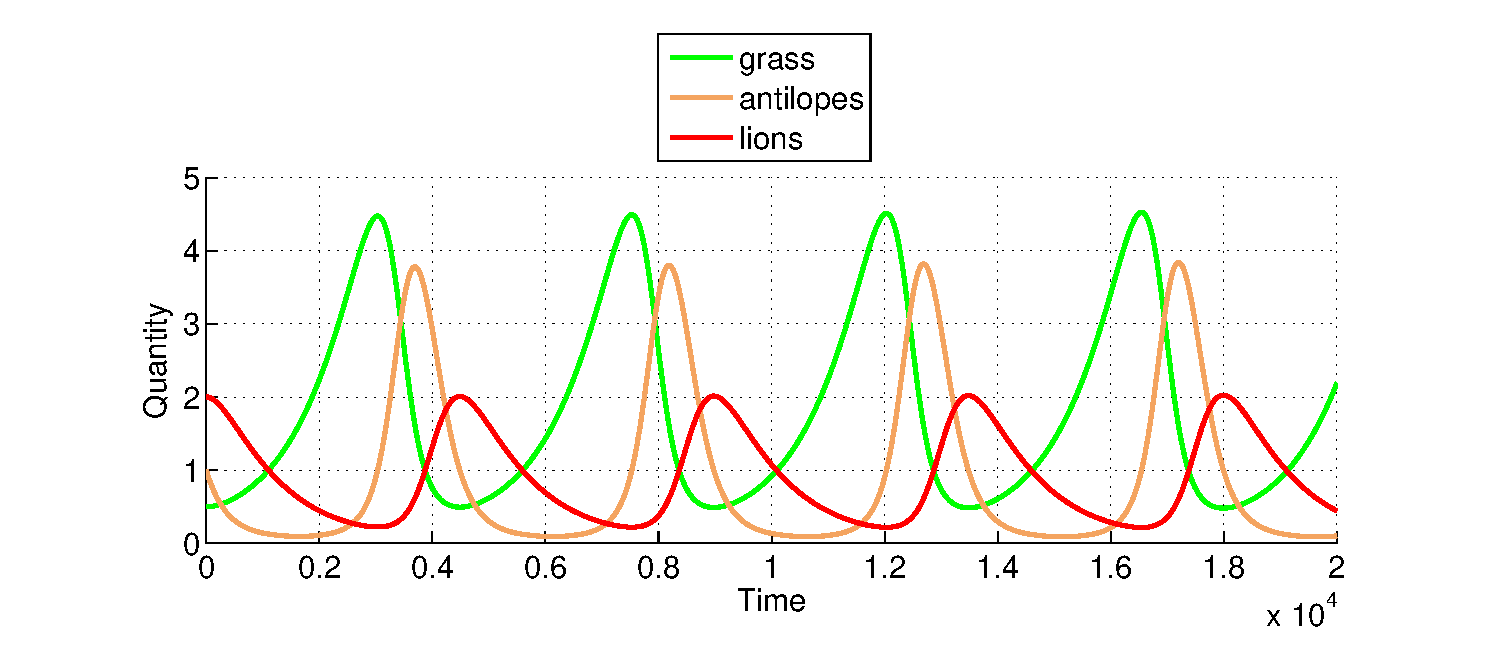
\includegraphics[scale=0.65]{LotkaVolterraThreeAllOnes.eps}
\caption{Lotka-Volterra equations for $a=b=c=d=e=f=g=1,start_X=0,5, start_Y=1,$ and $start_Z=2$.}
\label{fig:LotkaVolterraThreeAllOnes}
\end{figure}

\section{Simulation Results and Discussion}
Death by Age $\rightarrow$ increase reproduction Rate
Remove one species what happens
Location of animals have impact on survival, not only numbers
Cool pictures

%TODO: add parameters in CircleOfLife Code for nicely oscillating curves
Adjusting the parameters in the Lotka-Volterra formulas to the values shown in Table \ref{tab:LotkaVolterraParametersFinal} results in  population curves similar to the ones obtained from our simulation. Therefore, we conclude that our simulation models the habitat of organisms consistent to the Lotka-Volterra equations. 

\begin{table}[htbp]
\centering
\begin{tabular}{l|l}
Parameter & Value \\ 
\hline 
\hline
start\_X & 300\\
\hline
start\_Y & 30\\
\hline
start\_Z & 30\\
\hline
a & 0.075\\ 
\hline 
b & 0.0005\\ 
\hline 
c & 0.0005\\  
\hline 
d & 0.00025\\
\hline 
e & 0.0005\\
\hline 
f & 0.075\\
\hline 
g & 0.0005\\
\end{tabular}
\caption{The choice of constant values for the comparison with the simulation results}
\label{tab:LotkaVolterraParametersFinal}
\end{table}

The graphical result of the Lotka-Volterra equations for these parameters is shown in Figure \ref{fig:LotkaVolterraThreeAdjusted}.

\begin{figure}
\centering
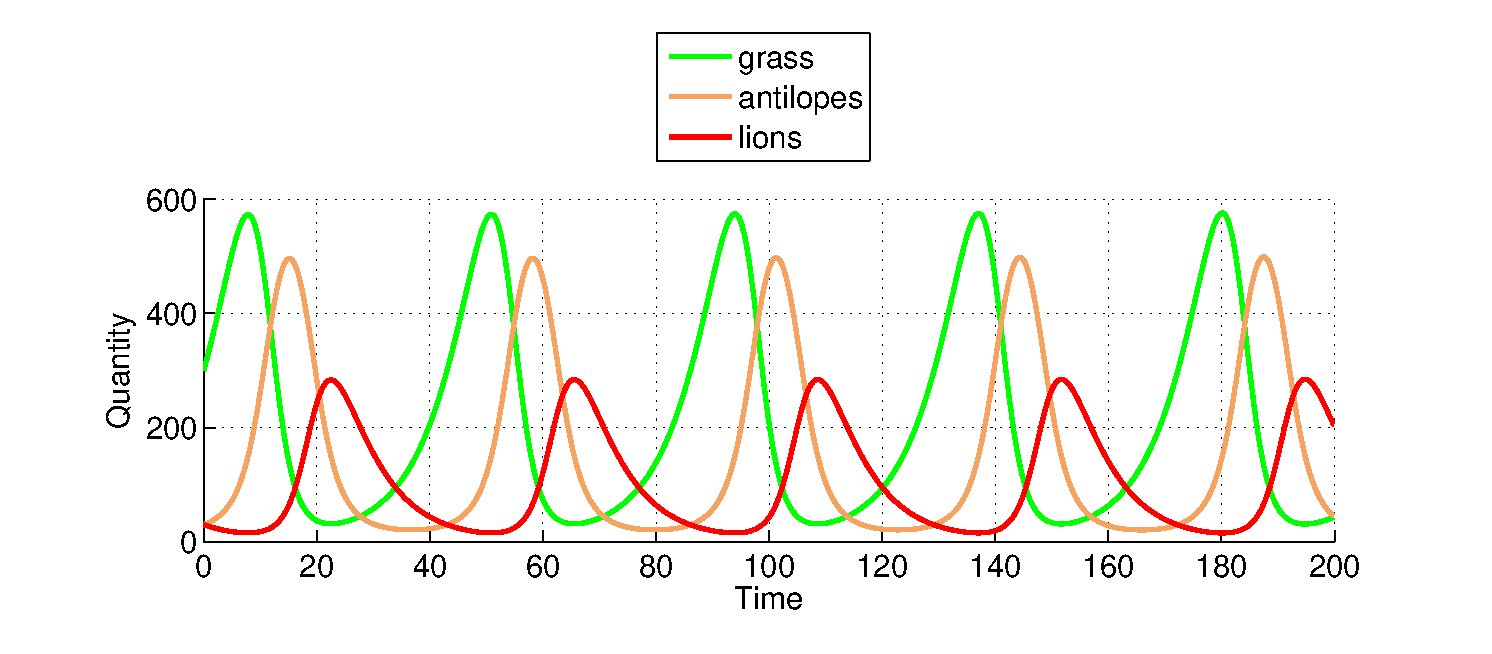
\includegraphics[scale=0.65]{LotkaVolterraThreeAdjusted.eps}
\caption{Lotka-Volterra equations for the parameters as shown in Table \ref{tab:LotkaVolterraParametersFinal}.}
\label{fig:LotkaVolterraThreeAdjusted}
\end{figure}

\section{Summary and Outlook}
Answer questions
Location of animals important. It is not taken into account by lotka-volterra.

Large Map size vs small map size
Size of "Wipeouts" is fix. Wipeout = one organism takes over. Small map oscillates more and will become unstable quicker. On large map multiple wipeouts can equalize each other.

Dependent of each other. 
Only antilipes and grass causes wipeout.

Large map equals stable non-oscillating cycle. 
Islands of Lions. Large Map results smaller probability of this happening. 
Antelopes become nothing, not grass


\appendix

\section{Appendix}
The title image was taken from \cite{titleImage}.

\section{Code}
%the final source code goes here

\bibliographystyle{plain}
\bibliography{bibliography}
\addcontentsline{toc}{chapter}{Bibliography}

\end{document}  